\documentclass{tudelft-report}

%% Set up the bibliography
\usepackage{biblatex}
\addbibresource{report.bib}

%% Additional packages and commands
\setlist{itemsep=-2pt} % Reducing white space in lists slightly
\renewcommand{\deg}{\si{\degree}\xspace} % Use \deg easily, everywhere

%% ----------------------------------------------------------------------
%%    Begin of document + Frontmatter (Roman page numbering)
%% ----------------------------------------------------------------------

\begin{document}

\frontmatter

%% Define the main parameters
\title{Algebra Topology}
\subtitle{learning note For reading translation}
\author{我真的不懂忧郁}

\subject{} % Cover only
\affiliation{Delft University of Technology} % Cover only
\coverimage{figures/cover.jpg} % Aspect ratio of 2:3 (portrait) recommended
\definecolor{title}{HTML}{4884d6} % Color for cover title

\makecover

\begin{titlepage}

\begin{center}

%% Print the title
{\makeatletter
\largetitlestyle\fontsize{45}{45}\selectfont\@title
\makeatother}

%% Print the subtitle
{\makeatletter
\ifdefvoid{\@subtitle}{}{\bigskip\titlestyle\fontsize{20}{20}\selectfont\@subtitle}
\makeatother}

\bigskip
\bigskip

by

\bigskip
\bigskip

%% Print the name of the author
{\makeatletter
\largetitlestyle\fontsize{25}{25}\selectfont\@author
\makeatother}

\bigskip
\bigskip

%% Print table with names and student numbers
\setlength\extrarowheight{2pt}
\begin{tabular}{lc}
    Student Name & Student Number \\\midrule
    First Surname & 1234567 \\
\end{tabular}

\vfill

%% Print some more information at the bottom
\begin{tabular}{ll}
    Instructor: & I. Surname \\
    Teaching Assistant: & I. Surname \\
    Project Duration: & Month, Year - Month, Year \\
    Faculty: & Faculty of Aerospace Engineering, Delft
\end{tabular}

\bigskip
\bigskip

%% Add a source and description for the cover and optional attribution for the template
\begin{tabular}{p{15mm}p{10cm}}
    Cover: & Canadarm 2 Robotic Arm Grapples SpaceX Dragon by NASA under CC BY-NC 2.0 (Modified) \\
    % Feel free to remove the following attribution, it is not required - still appreciated :-)
    Style: & TU Delft Report Style, with modifications by Daan Zwaneveld
\end{tabular}

\end{center}

%% Insert the TU Delft logo at the bottom of the page
\begin{tikzpicture}[remember picture, overlay]
    \node[above=10mm] at (current page.south) {%
        
\includegraphics{figures/logo-black}
    };
\end{tikzpicture}

\end{titlepage}

\chapter*{Preface}
\addcontentsline{toc}{chapter}{Preface}

\emph{A preface...}

\begin{flushright}
{\makeatletter\itshape
    \@author \\
    Delft, \monthname{} \the\year{}
\makeatother}
\end{flushright}









\chapter*{Summary}
\addcontentsline{toc}{chapter}{Summary}

\emph{A summary...}


\tableofcontents
%\listoffigures
%\listoftables

\chapter*{Nomenclature}
\addcontentsline{toc}{chapter}{Nomenclature}

\emph{If a nomenclature is required, a simple template can be found below for convenience. Feel free to use, adapt or completely remove.}

\section*{Abbreviations}

\begin{longtable}{p{2.5cm}p{8cm}}
    \toprule
    Abbreviation & Definition \\
    \midrule\endhead % Add abbreviations alphabetically here:
    ISA & International Standard Atmosphere \\
    ... \\
    \bottomrule
\end{longtable}

\section*{Symbols}

\begin{longtable}{p{2.5cm}p{8cm}p{2.5cm}}
    \toprule
    Symbol & Definition & Unit \\
    \midrule\endhead % Add Latin symbols alphabetically here:
    $V$ & Velocity & [m/s] \\
    ... \\
    \midrule % Add Greek symbols alphabetically here:
    $\rho$ & Density & [kg/m$^3$] \\
    ... \\
    \bottomrule
\end{longtable}


%% ----------------------------------------------------------------------
%%    Mainmatter (Arabic page numbering)
%% ----------------------------------------------------------------------

\mainmatter
    \chapter{高斯网络概述}

\section{概述}

\begin{center}
    \begin{forest}
        forest scheme
        [PGM
            [Bayes Network(有向图模型)]
            [MarKov Network(无向图模型)]
            [Gaussian Network
                [Gaussian Bayes Network(有向图模型)]
                [MarKov Bayes Network(有向图模型)]
            ]
        ]
    \end{forest}
\end{center}
    \chapter{\textsl{Base Group Exescrise}}

\section{道路同伦}

\begin{mdframed}
    \begin{question}
        空间$X$是\textbf{可缩}的,如果恒等映射$i_X:X\rightarrow X$是零伦的,
        \begin{enumerate}[itemindent=2em]
            \item 证明$I$和$\mathbb{R}$是可缩的;
            \item 证明可缩空间是道路连通的;
            \item 证明如果$Y$是可缩的,则对于任意的$X$,集合$[X,Y]$只有一个元素;
            \item 证明如果$X$是可缩的,并且$Y$是道路连通的,则$[X,Y]$只有一个元素;
        \end{enumerate}
    \end{question}
\end{mdframed}

\textbf{proof.}

$\Box$

\section{基本群}

\subsection*{\textsl{单连通性}}

\begin{mdframed}
    \begin{question}
        $\mathbb{R}^n$的一个子集$A$称为\textbf{星形凸集},如果$A$中有一个点$a_0$,使得链接$a_0$和$A$中任意另外一点的线段都包含在$A$中
        \begin{enumerate}[itemindent=2em]
            \item 找出一个不是凸集的星形凸集;
            \item 证明:若$A$是星形凸集,则$A$是单连通的;
        \end{enumerate}
    \end{question}
\end{mdframed}

\textbf{proof.}

$\Box$

\subsection*{\textsl{交换群}}

\begin{mdframed}
    \begin{question}
        设$x_0$和$x_1$是道路联通空间$X$中给定的两个点,证明:$\pi_1(X,x_0)$是一个交换群当且仅当对于任意两条从$x_0$到$x_1$的道路$\alpha$和$\beta$,有$\hat{\alpha}=\hat{\beta}$.
    \end{question}
\end{mdframed}

\textbf{proof.}

$\Box$

\subsection*{诱导同态}

\begin{mdframed}
    \begin{question}
        若$X$是道路连通的,则在不区别所设计的群之间的同构的前提下,连续映射的诱导同态与基点选择无关。(详细见p255 第6题)
    \end{question}
\end{mdframed}

\begin{mdframed}
    \begin{question}
        设$G$对于运算$*$而言是拓扑群,$x_0$使其单位元,令$\Omega(G,x_0)$表示$G$中以$x_0$为基点的所有回路的集合。若$f,g\in \Omega(G,x_0)$,定义一条回路$f\otimes g$,使得
        \begin{equation}
            (f\otimes g)(s)=f(s)*g(s)
        \end{equation}

        \begin{enumerate}[itemindent=2em]
            \item 证明这个运算使得集合$\Omega(G,x_0)$称为一个群;
            \item 证明这个运算在$\pi_1(G,x_0)$上诱导出一个群运算$\otimes$;
            \item 证明$\pi_1(G,x_0)$是一个交换群;
        \end{enumerate}
    \end{question}
\end{mdframed}


\section{覆叠空间}

\subsection*{\textsl{片状分拆}}

\begin{mdframed}
    \begin{question}
        设$p:E\rightarrow B$是连续的满射,$U$是$B$的一个被$p$均衡地覆盖着的开集,证明:如果$U$是连通的,则$p^{-1}(U)$的片状分拆是唯一的。
    \end{question}
\end{mdframed}

\subsection*{\textsl{k-重覆叠}}

\begin{mdframed}
    \begin{question}
        设$p:E\rightarrow B$是覆叠映射,又设$B$是连通的,证明:如果对于某一个$b_0\in B$,$p^{-1}(b_0)$恰好有$k$个元素,则对于每一个$b\in B$,$p^{-1}(b)$也恰好有$k$个元素。在这种情况下,$E$称为$B$的\textbf{k-重覆叠}。
    \end{question}
\end{mdframed}

\subsection*{\textsl{圆周$S^1$的覆叠空间}}

\begin{mdframed}
    \begin{question}
        证明例3中的映射是覆叠映射,并且将这个映射推广到$p(z)=z^n$
    \end{question}
\end{mdframed}

\subsection*{\textsl{紧致Hausdorff空间与覆叠映射}}

\begin{mdframed}
    \begin{question}
        设$p:E\rightarrow B$是覆叠映射
        \begin{enumerate}[itemindent=2em]
            \item 如果$B$是\textsl{Hausdorff}、正则、完全正则或者局部紧致的\textsl{Hausdorff}空间,则$E$满足同样的拓扑性质;
            \item 如果$B$是紧致的并且对于每一个$b\in B$,$p^{-1}(b)$是有限的,则$E$也是紧致的;
        \end{enumerate}
    \end{question}
\end{mdframed}

\section{圆周的基本群}

\subsection*{拓扑群}

\begin{mdframed}
    \begin{theorem}
        $S^1$的基本群同构于整数加群
    \end{theorem}
\end{mdframed}

\subsection*{\textsl{局部同胚}}

\begin{mdframed}
    \begin{question}
        对于53节例2中的局部同胚,“道路提升引理(引理54.1)”不能成立的理由是什么?
    \end{question}
\end{mdframed}

\subsection*{\textsl{道路提升}}

\begin{mdframed}
    \begin{question}
        设$p:E\rightarrow B$是覆叠映射,设$\alpha$和$\beta$是$B$中的道路,满足条件$\alpha(1)-\beta(0)$。又设$\tilde{\alpha}$和$\tilde{\beta}$是他们的提升,使得$\tilde{\alpha}(1)=\tilde{\beta}(0)$
        ,证明$\tilde{\alpha}*\tilde{\beta}$是$\alpha*\beta$的一个提升。
    \end{question}
\end{mdframed}

\subsection*{\textsl{环面的基本群}}

\begin{mdframed}
    \begin{question}
        推广定理54.5的证明,证明环面的基本群同构于群$\mathbb{Z}\times \mathbb{Z}$。
    \end{question}
\end{mdframed}

\section{收缩和不动点}

\subsection*{\textsl{圆盘的Brouwer不动点定理}}

\begin{mdframed}
    \begin{question}
        圆盘的Brouwer不动点定理证明
    \end{question}
\end{mdframed}

\begin{mdframed}
    \begin{question}(\textbf{Frobenius定理})
        设$A$是一个$3\times 3$正实数矩阵,则$A$有一个正的实特征值。
    \end{question}
\end{mdframed}

\begin{mdframed}
    \begin{question}
        证明如果$A$是非奇异的$3\times 3$非负矩阵,则$A$必有一个正的特征值。
    \end{question}
\end{mdframed}

\begin{mdframed}
    \begin{question}
        证明如果$A$是$B^2$的一个收缩核,则每一个连续映射$f:A\rightarrow A$必有一个不动点。
    \end{question}
\end{mdframed}

\subsection*{\textsl{收缩核}}

\begin{mdframed}
    \begin{question}
        假设对于每一个$n$,没有收缩$r:B^{n+1}\rightarrow S^n$,证明
        \begin{enumerate}[itemindent=2em]
            \item 恒等映射$i:S^n\rightarrow S^n$不是零伦的;
            \item 内射$j:S^n\rightarrow \mathbb{R}^{n+1}-\mathbf{0}$不是零伦的;
            \item $B^{n+1}$上每个非蜕化向量场必定在$S^n$的某一个点处指向圆心,在$S^n$某一点指向圆心的反方向;
            \item 每一个连续映射$f:B^{n+1}\rightarrow B^{n+1}$必然由一个不动点;
            \item 每一个由正实数组成的$(n+1)\times (n+1)$矩阵必然有正的特征根;
            \item 如果$h:S^n\rightarrow S^n$是零伦的,则$h$必然有一个不动点,同时$h$也将某一个点$x$映射为他的对径点$-x$。
        \end{enumerate}
    \end{question}
\end{mdframed}

\section{代数基本定理}

从圆周群计算的角度,证明代数学基本定理

\begin{mdframed}
    \begin{question}
        证明代数学基本定理:实系数或者复系数的$n>0$次方程
        \begin{equation}
            x^n+a_{n-1}x^{n-1}+\cdots+a_1x+a_0=0
        \end{equation}

        至少有一个实根或者复根
    \end{question}
\end{mdframed}

\begin{mdframed}
    \begin{question}
        证明实系数或者复系数的方程
        \begin{equation}
            x^n+a_{n-1}x^{n-1}+\cdots+a_1x+a_0=0
        \end{equation}

        当系数之和小于1时,这个方程所有根都在单位球$B^2$内部。
    \end{question}
\end{mdframed}

\section{Borsuk-Ulam定理}

\begin{mdframed}
    \begin{question}
        设$f:S^{n+1}\rightarrow \mathbb{R}^{n+1}$是一个连续映射,则$S^{n+1}$中必有一个点$x$使得$f(x)=-f(x)$。
    \end{question}
\end{mdframed}

\begin{mdframed}
    \begin{question}
        如果$A_1,\cdots,A_{n+1}$是$\mathbb{R}^{n+1}$中有界的可测集,则在$\mathbb{R}^{n+1}$中有一个$n$维平面平分这些集合中的每一个。
        \end{question}
\end{mdframed}

\begin{mdframed}
    \begin{question}
        在任何给定的时刻,地球表面上总有一对对径点,两处的温度和气压分别相同。
    \end{question}
\end{mdframed}

\section{形变收缩核和伦型}

书本281第3,5,6,9,10


\section{某些曲面的基本群}

\textbf{射影平面}$P^2$是$S^2$中等同每一个点$x$与它的对径点$-x$,而得到的商空间。

证明section 60所有的结论
    \chapter{Evaluation问题}

首先我们来整理一下现在所有的前提假设,首先我们有所有可能的状态变量$i_t$的状态集合$Q$和所有可能的状态变量$o_t$的观测集合$V$:

\begin{equation}
    Q=\{q_1,q_2,\cdots,q_N\}, \ \ \ \ V=\{v_1,v_2,\cdots,v_M\},
\end{equation}

其中$N$是可能的状态数,$M$是可能的观测数。

$I$是长度为$T$的状态序列,$O$是对应的观测序列:
\begin{equation}
    I=(I_1,I_2,\cdots,I_T),\ \ \ \ O=(O_1,O_2,\cdots,O_T)
\end{equation}

同时我们有参数$\lambda=(\pi,\mathcal{A},\mathcal{B})$,其中$\pi$为初始状态概率向量
\begin{equation}
    \pi = (\pi_i)_{N},\ \ \ \ \pi_i=P(I_1=q_i),\ i=1,2,\cdots,N
\end{equation}

$\mathcal{A}$是\textsl{状态转移矩阵},
\begin{equation}
    \mathcal{A}=[a_{ij}]_{N\times N}
\end{equation}

其中$a_{ij}=P(I_{t+1}=q_j|I_t=q_i)$。

$\mathcal{B}$是\textsl{观测概率矩阵},
\begin{equation}
    \mathcal{B}=[b_j(k)]_{N\times M}
\end{equation}

其中$b_{j}(k)=P(O_{t}=v_k|I_t=q_j)$。



\section{直接计算}

直接计算就是直接依照概率图模型直接展开,但是计算量很大,计算复杂度是$O(TN^T)$阶的。
\begin{equation}
    P(O|\lambda)=\sum_{I_1}\cdot\sum_{I_2}\cdot\cdots\cdot \sum_{I_T}\pi_{i_1}\prod_{t=2}^{T}a_{i_t-1,i_t}\prod_{t=2}^{T}b_{i_t}(O_t)
\end{equation}

一共有$T$个状态,每个状态$N$种可能,所以复杂度为$\mathcal{O}(N^T)$

\section{前向算法}


首先我们先展示一下Hidden Markov Model的拓扑结构
\begin{figure}[H]
    \centering
    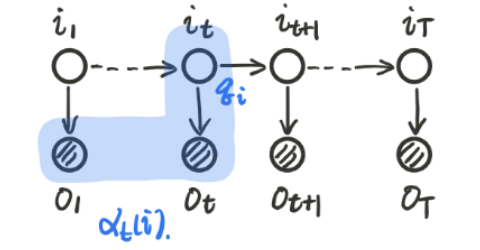
\includegraphics[scale=0.5]{figures/前向算法的拓扑结构.png}
    \caption{前向传播算法的拓扑结构}
\end{figure}

前向算法的主要思想是,在之前所有的观测变量$O_t$的前提下求出当前时刻的隐变量的概率,即
\begin{equation}
    P(O|\lambda)=\sum_{i=1}^{n} P(O,I_T=q_i|\lambda)=\sum_{i=1}^{n} \alpha_T(i)
\end{equation}

我们希望的是从$\alpha_1(i)$开始,一步一步向前推从而获得$\alpha_T$,也就是我们需要的是$\alpha_t(i)$和$\alpha_{t+1}(i)$具有某种递推关系,
下面我们来推导这种关系

\begin{mdframed}
    \begin{proposition}
        $\alpha_{t+1}(j)=b_j(O_{t+1})\cdot a_{ij}\cdot\alpha_i(i)$,其中$b_j(O_{t+1})=\sum_{k=1}^{M}\nu_k$
    \end{proposition}
\end{mdframed}

\begin{mdframed}[linewidth=0pt,backgroundcolor=gray!10]

    \begin{equation}
        \begin{aligned}
            \alpha_{t+1}(j)&=P(O_1,\cdots,O_t,O_{t+1},I_{t+1}=q_j|\lambda)\\
            &=\sum\limits_{i=1}^{N}P(O_1,\cdots,O_t,O_{t+1},I_{t}=q_i,I_{t+1}=q_j|\lambda)\\
            &=\sum\limits_{i=1}^{N}\underbrace{P(O_{t+1}|I_{t+1}=q_j,\lambda)}_{A}\underbrace{P(O_{1},O_{2},\cdots,O_{t},I_t=q_i,I_{t+1}=q_j|\lambda)}_{B}
        \end{aligned}
    \end{equation}

    其中$A$式刚好是观测概率矩阵的元素$b_j(O_{t+1})$

    \begin{equation}
        A=P(O_{t+1}|I_{t+1}=q_j,\lambda)=\sum_{k=1}^{M}b(O_{t+1}=\nu_k|I_{t+1=q_j},\lambda)=b_j(O_{t+1})
    \end{equation}

    主要来关注$B$,我们发现$B$还有关于$t+1$的项,我们想要这一项只和$t$及其之前的序列相关,因此对$B$做继续展开
    \begin{equation}
        \begin{aligned}
            B&=P(O_{1},O_{2},\cdots,O_{t},I_t=q_i,I_{t+1}=q_j|\lambda)\\
            &=P(I_{t+1}=q_j|O_{1},O_{2},\cdots,O_{t},I_t=q_i,\lambda)\cdot P(O_{1},O_{2},\cdots,O_{t},I_t=q_i|\lambda)\\
        \end{aligned}
    \end{equation}

    根据齐次马尔可夫假设
    \begin{equation}
        B=P(I_{t+1}=q_j|I_t=q_i,\lambda)\cdot P(O_{1},O_{2},\cdots,O_{t},I_t=q_i|\lambda)\\
    \end{equation}

    上式子左边第一项刚好是转移矩阵,第二项刚好是$\alpha_t(i)$所以
    \begin{equation}
        B=a_{ij}\cdot \alpha_t(i)
    \end{equation}

    然后我们把$A$和$B$最后的计算结果带回$\alpha_{t+1}(j)$
        \begin{equation}
            \alpha_{t+1}(j)=b_j(O_{t+1})\cdot a_{ij}\cdot \alpha_t(i)
        \end{equation}

\end{mdframed}

这个递推关系有什么意义呢?我们的联合概率分布是
\begin{equation}
    P(O|\lambda)=\sum_{i=1}^{n} P(O,I_T=q_i|\lambda)=\sum_{i=1}^{n} \alpha_T(i)
\end{equation}

利用递推关系,我们可以从简单的$\alpha_1$开始,用$\alpha_1$推导$\alpha_2$、$\alpha_2$推导$\alpha_3\cdots$,以此类推,最终算出来$\alpha_T(j)$,代入求和式就是联合概率分布。
而$\alpha_1$是只和一个状态结点和一个观测结点相关,因此是容易确定的。
\begin{figure}[H]
    \centering
    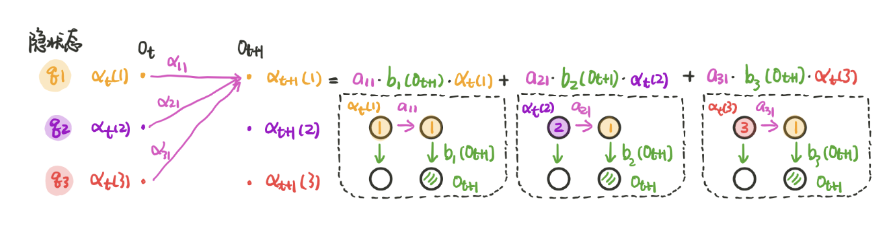
\includegraphics[scale=0.5]{figures/HMM前向传播示意图.png}
    \caption{HMM前向传播示意图}
\end{figure}

前向算法实际上是基于“状态序列的路径结构”递推计算联合概率分布的算法。其关键在于\textsl{局部计算前向概率,利用路径结构将前向概率递推到全局,从而减少每一次计算直接引用前一个时刻的计算结果,避免重复计算},
每次计算,隐状态的状态空间数为$N$,序列长度为$T$,因此这样利用前向计算算法的计算量是$O(N^2T)$阶的。


\section{后向算法}

后向概率的推导实际上比前向概率的理解要难一些,前向算法实际上是一个联合概率,而后向算法则是一个条件概率,所以后向的概率实际上比前向难求很多。

\begin{figure}[H]
    \centering
    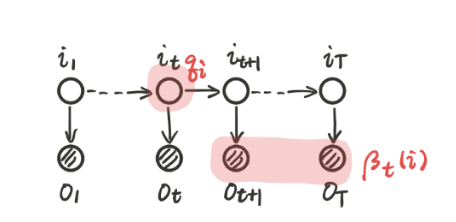
\includegraphics[scale=0.5]{figures/后向算法示意图2.png}
    \caption{后向算法示意图}
\end{figure}

我们设$\beta_{t}(i)=P(O_{t+1},\cdots,O_{T}|I_t=q_i,\lambda)$,计算观测的联合概率分布
\begin{equation}
    \begin{aligned}
        P(O|\lambda)&=P(O_1,O_2,\cdots,O_N|\lambda)\\
        &=\sum_{i=1}^{N}P(O_1,O_2,\cdots,O_N,I_1=q_i|\lambda)\\
        &=\sum_{i=1}^{N}P(O_1,O_2,\cdots,O_N|I_1=q_i,\lambda)\cdot P(I_1=q_i|\lambda)\\
        &=\sum_{i=1}^{N}P(O_1|O_2,\cdots,O_N,I_1=q_i|\lambda)\cdot P(O_2,\cdots,O_N,I_1=q_i|\lambda)\cdot\pi_i\\
        &=\sum_{i=1}^{N}P(O_1|I_1=q_i,\lambda)\cdot \beta_i(i)\cdot \pi_i\\
        &=\sum_{i=1}^{N}b_i(O_1)\cdot \beta_1(i)\cdot \pi_i
    \end{aligned}
\end{equation}

现在我们成功找到了$P(O|\lambda)$和第一个状态之间的关系,如下图所示
\begin{figure}[H]
    \centering
    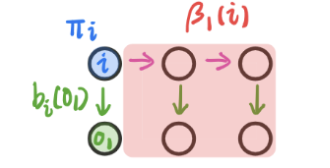
\includegraphics[scale=0.5]{figures/与第一个状态的关系.png}
    \caption{$P(O|\lambda)$与第一个状态的关系}
\end{figure}

现在我们要通过递推找最后一个状态和第一个状态的关系
\begin{equation}
    \begin{aligned}
        \beta_t(i)&=P(O_{t+1},\cdots,O_{T}|I_t=q_i)\\
        &=\sum_{j=1}^{N}P(O_{t+1},\cdots,O_{T}|I_t=q_i,i_{t+1}=q_j)\cdot P(I_{t+1}=q_j|I_t=q_i)
    \end{aligned}
\end{equation}

根据概率图模型,$I_t$和$t+1$后面所有的状态都没有关系,因此
\begin{equation}
    \begin{aligned}
        \beta_t(i)&=\sum_{j=1}^{N}P(O_{t+1},\cdots,O_T|I_{t+1}=q_j)\cdot a_{ij}\\
        &=\sum_{j=1}^{N}P(O_{t+1}|O_{t+1},\cdots,O_T,I_{t+1}=q_j)\cdot \underbrace{P(O_{t+2},\cdots,O_T|I_{t+1}=q_j)}_{\beta_{t+1}(j)}\cdot a_{ij}\\
        &=\sum_{j=1}^{N} b_j(O_{t+1})\cdot \beta_{t+1}(j)\cdot a_{ij}
     \end{aligned}
\end{equation}

马尔可夫链中每一个状态都是后一个状态的充分统计量,与之前的状态没有关系
\begin{equation}
    P(O_{t+1},\cdots,O_T|I_{t+1}=q_j,I_t=q_i)=P(O_{t+1},\cdots,O_T|I_{t+1}=q_j)
\end{equation}

通过这样的迭代方法从后往前推就可以得到$\beta_1(i)$的概率了,从而推断$P(O|\lambda)$。

\begin{figure}[H]
    \centering
    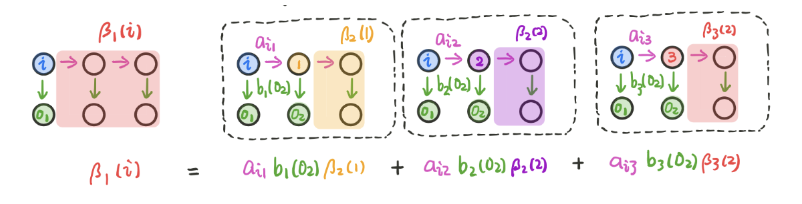
\includegraphics[scale=0.5]{figures/后向算法示意图.png}
    \caption{后向传播算法的拓扑结构}
\end{figure}
    \chapter{Normed Vector Space Exescrise}

\section{范数}

\begin{mdframed}
    \begin{question}
        设线性空间$X$中定义的距离$d$满足平移不变性和相似性,即$d(x+z,y+z)=d(x,y),d(\alpha x,\alpha y)=|\alpha|d(x,y)$,
        令$\Vert x\Vert=d(x,0)$,证明$(X,\Vert \cdot\Vert)$是赋范线性空间
    \end{question}
\end{mdframed}

\textbf{proof.} 如果$(X,\Vert\cdot\Vert)$是赋范线性空间,只要证明$\Vert\cdot\Vert$是$X$上的范数,只要证明满足三角不等式
\begin{equation}
    \begin{aligned}
        \Vert x+z\Vert&=d(x+z,-z+z)\\
        &=d(x,0)+d(-z,0)\\
        &=d(x,0)-d(z,0)\leqslant d(x,0)+d(z,0)=\Vert x\Vert+\Vert z\Vert
    \end{aligned} 
\end{equation}

PS:由两边之差小于第三边,两边之和大于第三边。

$\Box$

\section{\textsl{Banach}空间}

\begin{mdframed}
    \begin{question}
        在$\mathbb{C}^n$中定义范数$\Vert x\Vert=\max_{i}|x_i|$,证明他是\textsl{Banach}空间。
    \end{question}
\end{mdframed}

\textbf{proof.} 如果$\mathbb{C}^n$是\textsl{Banach}空间,则对于$\mathbb{C}^n$应该是完备的赋范空间,即$\mathbb{C}^n$中的所有\textsl{Cauchy}列都依范数收敛。
因此只要证明:$\forall \varepsilon>0$,存在一个$N\in \mathbb{N}$,使得对于所有的$k,m>N$
\begin{equation}
    \Vert x_k-x_m\Vert\leqslant \varepsilon
\end{equation}

其中$x_k=(x^{(1)}_k,x^{(2)}_k,\cdots,x^{(n)}_k),x_m=(x^{(1)}_m,x^{(2)}_m,\cdots,x^{(n)}_m)\in \mathbb{C}^n$。下面我们来证明,根据问题范数的定义
\begin{equation}
    \Vert x_k-x_m\Vert=\max\limits_{i}\ (x^{(i)}_k-x^{(i)}_m)
\end{equation}

问题就变成了$\mathbb{C}$中\textsl{Cauchy}序列收敛性问题,由于$\mathbb{C}$是完备的,因此总存在这样一个$N$使得问题满足。

$\Box$

\begin{mdframed}
    \begin{question}
        设$(X,\Vert\cdot\Vert)$是赋范空间,$X\neq\{0\}$,证明$X$为$Banach$空间的充要条件是$X$中单位球面$S=\{x\in X\ |\ \Vert x\Vert=1\}$
        是完备的。
    \end{question}
\end{mdframed}

\textsl{\textbf{分析}:$(1)$ 假设$\{x_k\}\in S$是单位球面上的\textsl{Cauchy}列,有$\lim_{k\rightarrow \infty}x_k=x$,注意$Cauchy$列和收敛的区别。$(2)$ $X$中任意的向量相当于单位向量的缩放:$v=x/\Vert x\Vert$ }

\textbf{proof.} 首先证明必要性。$X$是\textsl{Banach}空间,对于任意$S\subset X$上的\textsl{Cauchy}列,必然是收敛的。

再证明充分性。我们证明$X$中所有的\textsl{Cauchy}列收敛,取$\{y_n\}$是$X$中一组\textsl{Cauchy}列,由于$S$是完备的,则$\forall\ \varepsilon>0$,总存在$n$满足
\begin{equation}
    \Vert x_n-x\Vert=\Vert \frac{y_n}{\Vert y_n\Vert}-x\Vert<\frac{\varepsilon}{\Vert y_n\Vert}
\end{equation}

根据范数的齐次性
\begin{equation}
    \Vert y_n-\Vert y_n\Vert\cdot x\Vert<\Vert y_n\Vert\cdot \frac{\varepsilon}{\Vert y_n\Vert}=\varepsilon
\end{equation}

$\Box$

\begin{mdframed}
    \begin{question}
        设$H$是在直线$\mathbb{R}$上平凡可积,导数也平方可积的连续函数集合,对于每个$x\in H$,定义
        \begin{equation}
            \Vert x\Vert=\left(\int_{-\infty}^{\infty}|x(t)|^2dt+\int_{-\infty}^{\infty}|x'(t)|^2dt\right)
        \end{equation}

        证明$H$是\textsl{Banach}空间。
    \end{question}
\end{mdframed}

\textbf{proof.}

\begin{mdframed}
    \begin{question}
        设$0<p<1$,考虑空间$L^p[0,1]$,其中
        \begin{equation}
            \Vert x\Vert=\int_{0}^{1}|x(t)|^pdt<\infty,\ \ x\in L^p[0,1]
        \end{equation}

        证明$\Vert x\Vert$不是$L^p[0,1]$上的范数,但$d(x,y)=\Vert x-y\Vert$是$L^p[0,1]$上的距离。
    \end{question}
\end{mdframed}

\textbf{proof.}

\begin{mdframed}
    \begin{question}
        证明$l^p(1<p<\infty)$是可分的\textsl{Banach}空间。
    \end{question}
\end{mdframed}

\textsl{\textbf{分析}:$(1)$ $l^p$空间定义为$p$次方可求和的数列,
\begin{equation}
    l^p=\{x=\{\xi_n\}\ |\ \sum\limits_{n=1}^{\infty}|\xi_n|^p<\infty\}
\end{equation}
$(2)$可分:空间$X$可分意味着$X$中存在可数稠密子集$D$,即$X=\overline{D}$,即对于任意$x\in X$,以$x$为圆心任意半径的开球和$D$都有交集,即对于$X$中的每一个点都能用$D$中的序列去逼近。
$(3)$ $l^p$空间中可以赋予范数
\begin{equation}
    \Vert x\Vert_p=\left(\sum\limits_{n=1}^{\infty}|\xi_n|^p\right)^\frac{1}{p}
\end{equation}
}

\textbf{proof.} 

\begin{enumerate}[itemindent=2em]
    \item 证明$l^p$是\textsl{Banach}空间;
    
    如果$l^p$是\textsl{Banach}空间,则它应该是完备赋范空间,即对于任意的$l^p$中的\textsl{Cauchy}列,应该依照范数收敛于$l^p$中的某个值。
    ,考虑$l^p$空间中的一个\textsl{Cauchy}序列$\{x^{(n)}\}$,其中$x^{(n)}=(x^{(n)}_1,x^{(n)}_2,\cdots)$。所以对于$\forall\ \varepsilon>0$,
    $\exists\ N$,使得$\forall\ m,n>N$有
    \begin{equation}
        \Vert x^{(m)}-x^{(n)}\Vert_p=\left(\sum_{i=1}^{\infty}|x^{(m)}_i-x^{(n)}_i|^p\right)^{\frac{1}{p}}<\varepsilon
    \end{equation}

    对于每个$i$,$\{x^{(n)}_i\}$是$\mathbb{C}$中的\textsl{Cauchy}序列,所以它在$\mathbb{C}$中收敛于某个$x_i$,
    定义$x=(x_1,x_2,\cdots)$,我们证明$x\in l^p$,只要证明$x$的$p$次方可和。由于$x_1,x_2,\cdots$是有界数列,因此
    $x\in l^p$

    \item 证明$l^p$是可分的;设$D$为所有具有有限非零分量且分量是有理数的序列的集合,我们证明$D$在$l^p$中是可数稠密的。
    \begin{enumerate}[itemindent=2em]
        \item 由于有理数可数,所以$D$肯定是可数的;
        \item 证明$D$是稠密的,即证明对于任意$x\in X$以及任意的$\varepsilon>0$,存在$y\in D$,使得$\Vert x-y\Vert<\varepsilon$。
        \begin{equation}
            \Vert x-y\Vert<\Vert x-x^{(n)}\Vert+\Vert x^{(n)}-y\Vert
        \end{equation}
    \end{enumerate}
\end{enumerate}

$\Box$

\section{凸集}

\begin{mdframed}
    \begin{question}
        证明线性空间$X$中任何一族凸集的交集仍然是凸集;对任何$x_0\in X$,凸集$A$"移动"$x_0$后所得的集合$A+x_0=\{y+x_0\ |\ y\in A\}$仍然是凸集
    \end{question}
\end{mdframed}

\textbf{proof.}

\section{等距同构}

\begin{mdframed}
    \begin{question}
        设$C[0,1]$表示$(0,1]$上连续且有界的函数$x(t)$的全体,令
        \begin{equation}
            \Vert x\Vert=\sup\{x(t)\ |\ 0<t<1\}
        \end{equation}

        证明:
        \begin{enumerate}[itemindent=2em]
            \item $\Vert \cdot\Vert$是$C(0,1]$空间上的范数;
            \item $l^\infty$与$C(0,1]$的一个子空间等距同构;
        \end{enumerate}
    \end{question}
\end{mdframed}

\textbf{proof.}

\section{赋范空间上的连续映射}

\begin{mdframed}
    \begin{question}
        设$X$是一个赋范线性空间,且$X$中任意线性映射$L:X\rightarrow Y$连续,证明$X$是有限维的。
    \end{question}
\end{mdframed}

\textbf{proof.}

\section{最佳逼近}

\begin{mdframed}
    \begin{question}
        设$(X,\Vert\cdot\Vert)$是赋范空间,$Y$是$X$的子空间,对于$x\in X$,令
        \begin{equation}
            \delta = d(x,Y)=\inf_{y\in Y}\Vert x-y\Vert
        \end{equation}

        如果存在$y_0\in Y$,使得$\Vert x-y_0\Vert=\delta$,称$y_0$是$x$的最佳逼近
        \begin{enumerate}[itemindent=2em]
            \item 证明:如果$Y$是$X$的有限维子空间,则对于每个$x\in X$,存在最佳逼近;
            \item 证明:$Y$不是有限维空间时,上一个结论不成立;
            \item 证明:对于每一个点$x\in X$,$x$关于子空间$Y$的的最佳逼近点集是凸集;
        \end{enumerate}
    \end{question}
\end{mdframed}

\textbf{proof.}

\section{等价范数}

\begin{mdframed}
    \begin{question}
        设$(X_1,\Vert x\Vert_1),(X_2,\Vert x\Vert_2)$是赋范空间,在乘积线性空间$X_1\times X_2$中定义
        \begin{equation}
            \Vert z\Vert_1=\Vert x_1\Vert_1+\Vert x_2\Vert_2,\ \Vert z\Vert_2=\max\{\Vert x_1\Vert_1,\Vert x_2\Vert_2\},
        \end{equation}

        其中$z\in X_1\times X_2$,$z=(x_1,x_2)$,证明$\Vert\cdot\Vert_1,\Vert\cdot\Vert_2$是$X_1\times X_2$上的等价范数。
    \end{question}
\end{mdframed}

\section{赋范空间稠密与可分}

\begin{mdframed}
    \begin{question}
        设$(X,\Vert\cdot\Vert)$是赋范空间,$X_0$是$X$中的稠密子集,证明对于每个$x\in X$,存在$\{x_n\}\subset X_0$,使得
        \begin{equation}
            X=\sum_{n=1}^{\infty}x_n
        \end{equation}

        并且
        \begin{equation}
            \sum_{n=1}^{\infty}\Vert x_n\Vert<\infty
        \end{equation}
    \end{question}
\end{mdframed}

\textbf{proof.}

\begin{mdframed}
    \begin{question}
        设$X$是赋范线性空间,$M$是$X$闭子空间,证明若$X$可分,则$X/M$也可分。任取$y\in \overbrace{x}$,证明$\Vert \overbrace{x}\Vert=d(y,M)$。
    \end{question}
\end{mdframed}

\textbf{proof.}

\begin{mdframed}
    \begin{question}
        设$X$是赋范线性空间,$M$是$X$的闭子空间,如果$M$以及$X/M$是\textsl{Banach}空间,证明$X$也是\textsl{Banach}空间。
    \end{question}
\end{mdframed}

\textbf{proof.}

    \chapter{\textsl{Lagrange}力学}

\section{广义坐标}

\section{最小作用量原理}

使得泛函最小
\begin{equation}
    S[\mathcal{L}(q,\dot{q},t)]=\int_{t_1}^{t_2} \mathcal{L}(q(t),\dot{q}(t),t) dt
\end{equation}

\section{\textsl{Lagrange}方程}

由泛函的一阶变分并根据泛函极值条件可得拉格朗日方程
\begin{equation}
    \frac{\partial\ \mathcal{L}}{\partial q}-\frac{d}{dt}(\frac{\partial\ \mathcal{L}}{\partial \dot{q}})=0
\end{equation}

\section{对称量与守恒量}

在物理学中有三个基本的守恒量

\begin{enumerate}[itemindent=2em]
    \item 时间平移对称性$\ \Rightarrow\ $能量守恒;
    \item 空间平移对称性$\ \Rightarrow\ $动量守恒;
    \item 空间旋转对称性$\ \Rightarrow\ $角动量守恒;
\end{enumerate}

诺特定理给守恒量的存在提供了理论基础。

\begin{framed}
    \begin{theorem}
        (\textbf{诺特定理}) 如果系统的拉格朗日量在连续的连续无穷小变换$q\rightarrow q'=q'(\epsilon)$($\epsilon$是一阶小量)下保持不变,
        \begin{equation}
            \mathcal{L}(q(\epsilon),\dot{q}'(\epsilon),t)-\mathcal{L}(q,\dot{q},t)=0\ \Leftrightarrow\ \left.\frac{\partial \mathcal{L}(q(\epsilon),\dot{q}'(\epsilon))}{\partial \epsilon}\right|_{\epsilon=0}=0
        \end{equation}
        则系统必存在守恒量
        \begin{equation}
            \varLambda=\frac{\partial \mathcal{L}}{\partial \dot{q}}\left.\frac{d q'}{d \epsilon}\right|_{\epsilon=0}
        \end{equation}
    \end{theorem}
\end{framed}

\footnote{如果一个系统的拉格朗日量对于某个广义坐标$q_i$不显含(即对称性存在),那么对应的广义动量$p_i$是守恒的。}
\begin{mdframed}[backgroundcolor=gray!20,hidealllines=true]
    \textbf{proof}. 根据在连续无穷小变换下保持不变
    \begin{equation}
        \begin{aligned}
            \left.\frac{\partial \mathcal{L}(q(\epsilon),\dot{q}'(\epsilon))}{\partial \epsilon}\right|_{\epsilon=0}&=\left[\frac{\partial\mathcal{L}}{\partial q'}\frac{\partial q'}{\partial \epsilon}+\frac{\partial\mathcal{L}}{\partial \dot{q}'}\frac{\partial \dot{q}'}{\partial \epsilon}\right]_{\epsilon=0}=0
        \end{aligned}
     \end{equation}

     由欧拉-拉格朗日方程得到
     \begin{equation}
        \frac{d}{dt}(\frac{\partial\mathcal{L}}{\partial \dot{q}'})\cdot\frac{d q'}{d\epsilon}+\frac{\partial \mathcal{L}}{\partial \dot{q}'}\cdot \frac{d \dot{q}}{d\epsilon}=0
     \end{equation}

     因此
     \begin{equation}
        \frac{d}{dt}\left[\frac{\partial\mathcal{L}}{\partial \dot{q}'}\cdot \frac{dq'}{d\epsilon}\right]=0\ \Rightarrow\ \left.\frac{\partial\mathcal{L}}{\partial \dot{q}'}\cdot \frac{dq'}{d\epsilon}\right|_{\epsilon=0}=\varLambda
     \end{equation}

\end{mdframed}


这是诺特定理最简单的表述,他告诉我们如果一个作用量做没有外界给予的突变的情况下,一定存在一个守恒量。下面验证一下前面描述的三种变换下守恒量存在。

\subsection*{能量守恒}

首先在\textsl{时间均匀性},推出能量守恒定律,由于时间均匀,即时间平动下拉格朗日量形式保持不变,因此拉格朗日量不显含时间,因此
\begin{equation}
    \frac{d \mathcal{L}}{dt}=\frac{\partial \mathcal{L}}{\partial \dot{q}}\cdot \frac{\partial \dot{q}}{\partial t}+\frac{\partial \mathcal{L}}{\partial q}\cdot \frac{\partial q}{\partial t}
\end{equation}

根据\textsl{Euler-Lagrange方程},上面式子可以化为

\begin{equation}
    \frac{d}{dt}\left[\frac{\partial \mathcal{L}}{\partial \dot{q}}\cdot \frac{\partial q}{\partial t}\right]=\frac{d\mathcal{L}}{dt}
    \ \Rightarrow\ \frac{d}{d}\left[\frac{\partial \mathcal{L}}{\partial \dot{q}}\cdot \frac{\partial q}{\partial t}-\mathcal{L}\right]=0
\end{equation}

最终得到
\begin{equation}
    \varLambda=\dot{q}\cdot\frac{\partial\mathcal{L}}{\partial\dot{q}}-\mathcal{L}
    \label{eq3.10}
\end{equation}

封闭系统的拉格朗日量一般可以表述为
\begin{equation}
    \mathcal{L}=\frac{1}{2}m\dot{q}^2-U(q)
\end{equation}

代入(\ref{eq3.10}),得到
\begin{equation}
    m\dot{q}^2-\mathcal{L}=\frac{1}{2}m\dot{q}^2+U(q)=E
\end{equation}

这刚好是机械能守恒。


\subsection*{动量守恒}

\textsl{空间平移对称性}意味着拉格朗日量不显含有广义坐标$q$,由\textsl{Euler-Lagrange方程}有
\begin{equation}
    \frac{d}{dt}\left[\frac{\partial \mathcal{L}}{\partial \dot{q}}\right]=\frac{\partial \mathcal{L}}{\partial q}=0
\end{equation}

即
\begin{equation}
    \frac{\partial \mathcal{L}}{\partial \dot{q}}=p=Constant
\end{equation}

$p$我们常常称之为\textsl{广义动量}。例如势能场中的运动例子
\begin{equation}
    \mathcal{L}=\frac{1}{2}mv^2-U(r)
\end{equation}

广义坐标为位移$r$,则广义动量为
\begin{equation}
    p=\frac{\partial \mathcal{L}}{\partial v}=mv
\end{equation}

这刚好是线性动量一般的表达式。广义动量不仅能描述线性动量,也能描述角动量,考虑在二维平面势能场中运动的粒子,

\subsection*{角动量守恒}

角动量守恒描述的是\textsl{空间各向同性},注意到我们前面定义的变分是关于空间位移的变分$\delta r=r_1(t)-r_2(t)$,现在我们要换成旋转位移的变分$\delta \varphi=\varphi_1(t)-\varphi_2(t)$,根据最小作用量原理和泛函极值条件
\begin{equation}
    \delta \mathcal{L}=\frac{\partial \mathcal{L}}{\partial r}\delta r+\frac{\partial \mathcal{L}}{\partial \dot{r}}\delta \dot{r}=0
\end{equation}

我们把$\delta r$替换成和角度相关的量
\begin{equation}
    \begin{aligned}
        & \delta r=r\times \delta \varphi\\
        & \delta\dot{r} =\dot{r}\times \delta \varphi\\
    \end{aligned}
\end{equation}

再由拉格朗日方程
\begin{equation}
    \begin{aligned}
        & \frac{\partial \mathcal{L}}{\partial \dot{r}}=p\\
        & \frac{\partial \mathcal{L}}{\partial r}=\dot{p}\\
    \end{aligned}
\end{equation}

整理得到
\begin{equation}
    \delta \mathcal{L}=p\cdot(\dot{r}\times \delta\varphi)+\dot{p}\cdot(r\times \delta \varphi)=0
\end{equation}

注意这里$p,r,\varphi$都是矢量,那么根据矢量运算法则,可以把$\delta\varphi$提出得到
\begin{equation}
    \delta \varphi\cdot(r\times \dot{p}+\dot{r}\times p)=\delta \varphi\cdot\frac{d}{dt}\left[(r\times p)\right]=0
\end{equation}

由$\delta\varphi$的任意性,所以只能是对时间的导数项为$0$,即
\begin{equation}
    r\times p=\mathcal{M}=Constant
\end{equation}

这里向量$\mathcal{M}$称之为\textsl{角动量}。角动量守恒的条件为外力矩为零。


\section{条件极值}

如果泛函极值存在约束条件,往往是以下的形式
\begin{equation}
    f(q,\dot{q},t)=0
\end{equation}

由拉格朗日乘子法,构造新的泛函
\begin{equation}
    \mathcal{H}(q(t),\dot{q}(t),t)=\mathcal{L}(q(t),\dot{q}(t),t)+\lambda^T f(q,\dot{q},t)
\end{equation}

其中$\lambda(t)=(\lambda_1(t),\lambda_2(t),\cdots,\lambda_n(t))$,分别求导可得
\begin{equation}
    \left\{ 
        \begin{aligned}
        & \frac{\partial \mathcal{H}}{\partial q}-\frac{d}{dt}\cdot \frac{\partial \mathcal{H}}{\partial \dot{q}}=0\\
        & \frac{\partial \mathcal{H}}{\partial \lambda}-\frac{d}{dt}\cdot \frac{\partial \mathcal{H}}{\partial \dot{\lambda}}=f=0
    \end{aligned}
    \right.
\end{equation}


    \chapter{\textsl{Hilbert Space Exescrise}}

稍微记录一下:度量和内积的关系在于,由于度量描述的是距离,对于任意两个点之间的距离都应该用一个正数表示,内积是有可能是负的,代表角度大于90度;度量是一个泛函而内积是一个双线性泛函,就是说度量不一定满足线性;同时度量遵守的是三角不等式量定义了“距离”并且必须满足最基本的几何直觉,即从一处到另一处的直接距离不能超过绕道的距离和,而内积遵守平行四边形不等式,内积不仅定义了距离,还定义了角度和正交性。平行四边形不等式是由向量加法和内积定义的范数之间的关系决定的,它描述了内积空间中的几何对称性。

\textbf{总结:}由度量$d(\cdot,\cdot)$诱导的范数只能描述距离,而内积诱导的范数可以描述角度和距离。
\begin{equation}
    (x,y)=\Vert x\Vert\Vert y\Vert\cos\theta
\end{equation}


\section{用内积生成的范数}

% question 25 
\begin{mdframed}
    \begin{question}
        至少举例两个线性赋范空间$X$,使得在$X$上的范数不能由内积生成
    \end{question}
\end{mdframed}

\textbf{proof.}

$\Box$

\section{\textsl{Hilbert}空间收敛性}

% question 26
\begin{mdframed}
    \begin{question}
        设$\{x_n\}$为内积空间$H$中点列,$x\in H$,若$\Vert x_n\Vert\rightarrow \Vert x\Vert$,且$\forall\ y\in H$,$(x_n,y)\rightarrow (x,y)\ (n\rightarrow \infty)$,证明:$x_n\rightarrow x\ (n\rightarrow \infty)$
    \end{question}
\end{mdframed}

\textbf{proof.}

$\Box$

% question 27
\begin{mdframed}
    \begin{question}
        设$H$是\textsl{Hilbert}空间,$\{x_n\}\subset H$,满足$\sum_{n=1}^{\infty}\Vert x_n\Vert<\infty$,证明$\sum_{n=1}^{\infty}x_n$在$H$中收敛。
    \end{question}
\end{mdframed}

\textbf{proof.}

$\Box$

\section{可分的\textsl{Hilbert}空间}

% question 28
\begin{mdframed}
    \begin{question}
        证明在可分的内积空间,任意标准正交系最多为一可数集
    \end{question}
\end{mdframed}

\textbf{proof.}

$\Box$

% question 29
\begin{mdframed}
    \begin{question}
        证明在可分的\textsl{Hilbert}空间中,任一完备的标准正交系必定是可数集
    \end{question}
\end{mdframed}

\textbf{proof.}

$\Box$

\section{\textsl{Hilbert}空间正交系与正交基}

% question 30
\begin{mdframed}
    \begin{question}
        设$E_n$是$n$为实线性空间,$\{e_1,e_2,\cdots,e_n\}$是$E_n$的一个基,$(\alpha_{ij})(i,j=1,2,\cdots,n)$是正定矩阵,对$E_n$中的元素$x=\sum\limits_{i=1}^{n}x_ie_i$以及$y=\sum\limits_{i=1}^{n}y_ie_i$,定义
        \begin{equation}
            (x,y)=\sum_{i,j=1}^{n}x_i\alpha_{ij}y_j
        \end{equation}

        证明:$(\cdot,\cdot)$是$E_n$上的一个内积,反之,设$(\cdot,\cdot)$是$E_n$上的一个内积,则必定存在正定矩阵$(\alpha_{ij})$使得$(x,y)=\sum x_i\alpha_{ij} y_j$成立。
    \end{question}
\end{mdframed}

\textsl{\textbf{分析}:(1)内积本质上是一个双线性函数,满足正定性,共轭对称性,线性性;$(2)$ 正定矩阵:如果一个$n\times n$的实对称矩阵是正定的,当且仅当对于所有的非零实系数向量$z$,都有$z^TMz>0$;}

\textbf{proof.} 证明如下

\textbf{step 1.} 首先证明$(\cdot,\cdot):E_n\times E_n\rightarrow \mathbb{R}$是$E_n$上的一个内积。将内积形式写成矩阵形式,令$A=(\alpha_{ij})_{n\times n}$

\begin{equation}
    (x,y)=xAy
\end{equation}

\begin{enumerate}[itemindent=2em]
    \item 正定性:取$x\in E_n$,由于$A$是正定实对称矩阵
    \begin{equation}
        xAx^T\geqslant 0
    \end{equation}

    当且仅当$\Vert x\Vert=0$时等号满足
    \item 线性性:
    \begin{equation}
        \begin{aligned}
            & (\alpha x,\beta y)=(\alpha x)A(\beta y)=\alpha(xAy)\beta=a\\
            & (x+z,y)=(x+z)Ay=xAy+zAy=(x,z)+(x,y)\\
        \end{aligned}
    \end{equation}
    \item 对称性:由于$(\cdot,\cdot)$是一个双线性函数,输出是一个实数,转置前后结果不变,同时$A$对称,所以
    \begin{equation}
        (x,y)=xAy=(xAy)^T=y^TAx^T=(y,x)
    \end{equation}
\end{enumerate}

\textbf{step 2.} 如果$(\cdot,\cdot)$是$E_n$上的一个内积,对于任意的$\mathbf{x},\mathbf{y}\in E_n$
\begin{equation}
    \begin{aligned}
        (\mathbf{x},\mathbf{y})&=(\sum_{i=1}^{n}x_ie_i,\sum_{j=1}^{n}y_je_j)
        &=\sum_{i=1}^{n}\sum_{j=1}^{n}x_i(e_i,e_j)y_j
    \end{aligned}
\end{equation}

令$\alpha_{ij}=(e_i,e_j)$,再令
\begin{equation}
    A=\left[
        \begin{array}{ccccc}
            (e_1,e_1) & (e_1,e_2) & \cdots & (e_1,e_n) \\
            (e_2,e_1) & (e_2,e_2) & \cdots & (e_2,e_n) \\
            \vdots    & \vdots    & \ddots & \vdots    \\
            (e_n,e_1) & (e_n,e_2) & \cdots & (e_n,e_n) \\
        \end{array}
    \right]
\end{equation}

下面只要证明$A$是一个正定矩阵,首先注意到$A$是一个实对称矩阵,如果$A$是一个正定矩阵,则$\forall\ \mathbf{z}\in E_n$
\begin{equation}
    \mathbf{z}A\mathbf{z}^T=\sum_{i=1}^{n}\sum_{j=1}^{n}z_i\alpha_{ij}z_j=(\mathbf{z},\mathbf{z})=\Vert \mathbf{z}\Vert^2>0(\mbox{由内积诱导范数})
\end{equation}

\textsl{PS:上面的矩阵$A$实系数下称为Gram矩阵。}

$\Box$

% question 31
\begin{mdframed}
    \begin{question}
        称$H_n(t)=(-1)^ne^{t^2}\frac{d^n}{dt^n}e^{-t^2}$为\textsl{Hermite}多项式,令
        \begin{equation}
            e_n(t)=(2^nn!\sqrt{\pi})^{-\frac{1}{2}}e^{-\frac{t^2}{2}}H_n(t)\ \ \ \ (n=1,2,\cdots)
        \end{equation}

        证明$\{e_n\}$组成$L^2(-\infty,\infty)$中的一个完备标准正交基
    \end{question}
\end{mdframed}

\textbf{proof.}

$\Box$

% question 32
\begin{mdframed}
    \begin{question}
        令$L_n(t)$为\textsl{Laguerre}函数$e^t\frac{d^n}{dt^n}(t^ne^{-t})$,证明$\{\frac{1}{n!}e^{-\frac{1}{2}}L_n(t)\}(n=1,2,\cdots)$组成的$L^2(0,\infty)$中的一个完备的标准正交基
    \end{question}
\end{mdframed}

\textbf{proof.}

$\Box$

\section{正交补空间}

% question 33
\begin{mdframed}
    \begin{question}
        设$M=\{x|x=\{\xi_n\}\in l^2,\xi_{2n}=0,n=1,2,\cdots\}$,证明$M$是$l^2$的闭子空间,且求出$M^\perp$
    \end{question}
\end{mdframed}

\textsl{\textbf{分析:} 证明$l^p$空间完备性的时候,是证明$x=(\xi_1,\xi_2,\cdots)\in l^p$的每一个分量$\xi_i$在$\mathbb{C}$中的收敛性,根据点集拓扑学中积空间的讨论,$l^p$可以看作$\mathbb{C}\times \mathbb{C}\times \cdots$笛卡尔积的形式,根据点集拓扑学中积空间的讨论,如果$x$的分量$\xi_i$在$\mathbb{C}$中收敛,那么$x$在$l^p$收敛。} 

\textbf{proof.} 首先证明$M$是$l^2$是闭集;首先$l^2$空间上的范数定义为
\begin{equation}
    \Vert x\Vert :=\left(\sum_{k=1}^{\infty} |\xi_k|^2\right)^\frac{1}{2}
\end{equation}

如果$M$是闭集,则对于任意$x\in M$,那么存在任意的$B(x,\varepsilon)$和$M$的交集都不为空,也就是说存在一个序列$\{x^{(k)}\}\in M$,使得
\begin{equation}
    \Vert x^{(k)}-x\Vert<\varepsilon,\ \ \ \forall\ \varepsilon>0
\end{equation}

其中$x^{(k)}=(\xi^{(k)}_1,0,\xi^{(k)}_3,0,\cdots)$,$x=(\xi_1,0,\xi_3,0,\cdots)$,根据依照范数收敛的定义,上面写成
\begin{equation}
    \left(\sum_{n=1}^{\infty} |\xi^{(k)}_{2n-1}-\xi_{2n-1}|^2\right)^\frac{1}{2}<\varepsilon
\end{equation}

同时知道$l^p$空间在范数拓扑的情况下可分,因此$l^p$空间的任意一个点都至少存在一个收敛到它的序列。假设存在$\{y^{(k)}\}\in l^2$刚好收敛到$x$,其中$y^{(k)}=(\xi^{(k)}_1,\xi^{(k)}_2,\xi^{(k)}_3,\xi^{(k)}_4,\cdots)$则

\begin{equation}
    \left(\sum_{n=1}^{\infty} |\xi^{(k)}_{n}-\xi_{n}|^2\right)^\frac{1}{2}<\varepsilon
\end{equation}

这相当于是填补了偶数项,所以
\begin{equation}
    \left(\sum_{n=1}^{\infty} |\xi^{(k)}_{2n-1}-\xi_{2n-1}|^2\right)^\frac{1}{2}< \left(\sum_{n=1}^{\infty} |\xi^{(k)}_{n}-\xi_{n}|^2\right)^\frac{1}{2}<\varepsilon
\end{equation}

所以对于任意的$x\in M$,包含$x$所有的开球$B(x,\varepsilon)\cap M\neq \emptyset$。所以$M$闭。

下面求$M$的正交补空间。定义$l^2$上的内积为
\begin{equation}
    (x,y)=\sum_{n=1}^{\infty} \eta_n\overline{\xi_n}
\end{equation}

正交补空间的定义为

\begin{equation}
    M^\perp =\{x\in l^2|(x,y)=0,\forall\ y\in M\}
\end{equation}

令$x=(\xi_1,\xi_2,\cdots)\in l^2$,$y=(\eta_1,\eta_2,\cdots)\in M$,其中$y$的偶数项全都为$0$,我们来找$x$
\begin{equation}
    (x,y)=\sum_{n=1}^{\infty} \sum_{n=1}^{\infty} \eta_{2n-1}\overline{\xi_{2n-1}}=0
\end{equation}

因为奇数项全部为$0$,所以上面只有奇数项,而奇数项$\xi_i$又不全为$0$,所以上式如果对于任意的$y$都满足,当且仅当$x$在奇数的分量全部为$0$。所以
\begin{equation}
    M^\perp =\{x\in l^2|x=\{\xi_1,\xi_2,\cdots\},\xi_{2n-1}=0,n=1,2,\cdots\}
\end{equation}

$\Box$

% question 34
\begin{mdframed}
    \begin{question}
        设$X$是内积空间,$A\subset X$,证明$A^\perp=\overline{A}^\perp$
    \end{question}
\end{mdframed}

\textsl{\textbf{分析}:注意正交补空间的定义是,在正交补空间中每一个元素和原子空间的每个元素都相互正交}

\textbf{proof.} $A$的正交补空间定义为
\begin{equation}
    A^\perp=\{x\in X|(x,y)=0,\forall y\in A\}
\end{equation}
\begin{equation}
    \overline{A}^\perp=\{x\in X|(x,y)=0,\forall y\in \overline{A}\}
\end{equation}

\begin{enumerate}[itemindent=2em]
    \item 证明$A^\perp \subseteq \overline{A}^\perp$;

    如果$A^\perp \subseteq \overline{A}^\perp$,则对于所有的$y\in A^\perp$,任意取在$X$中收敛的数列$\{x_k\}\subseteq A$,
    \begin{equation}
        (x_k,y)=0
    \end{equation}

    令$k\rightarrow \infty$,根据内积的连续性
    \begin{equation}
        \lim_{k\rightarrow \infty}(x_k,y)=\lim_{k\rightarrow \infty}(x_k,y)=(x,y)=0
    \end{equation}

    因为$\overline{A}$包含$A$和$A$的所有的极限点,所以$x\in \overline{A}$。也就是说$y\in \overline{A}^\perp$,由于$y$的任意性,所以
    \begin{equation}
        A^\perp\subseteq \overline{A}^\perp
    \end{equation}

    \item 证明$\overline{A}^\perp \subseteq A^\perp$;
    
    假设$y\in \overline{A}^\perp$,对于任意的$x\in \overline{A}$,都有
    \begin{equation}
        (x,y)=0
    \end{equation}

    由于$A\subseteq \overline{A}$,所以对于任意的$z\in A$,也都有
    \begin{equation}
        (z,y)=0
    \end{equation}

    也就是说$y\in A^\perp$,所以$\overline{A}^\perp \subseteq A^\perp$。
\end{enumerate}

综上所述,$A^\perp=\overline{A}^\perp$

$\Box$

% question 35
\begin{mdframed}
    \begin{question}
        设$M,N$是内积空间$H$的子空间,$M\perp N$,$L=M\bigoplus N$,证明$L$是闭子空间的充分必要条件是$M,N$均为闭子空间(充分性部分假定$H$完备)。
    \end{question}
\end{mdframed}

\textbf{proof.}

$\Box$

\section{\textsl{Fouries}级数}

% question 36
\begin{mdframed}
    \begin{question}
        试证:$\left\{\sqrt{\frac{2}{\pi}}\sin\ nt\right\}$构成$L^2[0,2\pi]$的正交基,但不是$L^2[-\pi,\pi]$的正交基。
    \end{question}
\end{mdframed}

\textbf{proof.}

$\Box$

% question 37
\begin{mdframed}
    \begin{question}
        设$H$表示如下的函数$x(t)$的全体
        \begin{equation}
            x(t)\in L[0,2\pi],x(t)\sim \frac{a_0}{2}+\sum_{n=1}^{\infty}(a_n\cos nt+b_n\sin nt)
        \end{equation}

        且
        \begin{equation}
            \sum_{n=1}^{\infty}n(a^2_n+b^2_n)<\infty
        \end{equation}

        令
        \begin{equation}
            \Vert x\Vert_H=\frac{1}{\pi}\left[\frac{a_0^2}{2}+\sum_{n=1}^{\infty}n(a^2_n+b^2_n)\right]^\frac{1}{2}
        \end{equation}

        证明$H$是\textsl{Hilbert}空间。
    \end{question}
\end{mdframed}

\textbf{proof.}

$\Box$

\section{凸性}

% question 38
\begin{mdframed}
    \begin{question}
        赋范线性空间$X$被称为一致凸的,如果$X$中任意满足$\Vert x_n\Vert=\Vert y_n\Vert=1,\Vert x_n+y_n\Vert\rightarrow 2$的序列$\{x_n\},\{y_n\}$有$\Vert x_n-y_n\Vert\rightarrow 0$,证明:
        \begin{enumerate}[itemindent=2em]
            \item 任何内积空间都是一致凸的;
            \item $C[a,b]$不是一致凸的;
            \item $L^1[a,b]$不是一致凸的;
            \item 一致凸赋范空间必然是严格凸的;
        \end{enumerate}
    \end{question}
\end{mdframed}

\textbf{proof.}

$\Box$

\section{正交投影与最佳逼近}

\begin{mdframed}
    \begin{question}
        证明在严格凸的赋范空间中,对于每个$xin X$,$x$关于任意闭子空间$Y$的最佳逼近都是唯一的。
    \end{question}
\end{mdframed}

\begin{mdframed}
    \begin{question}
        设$H$是\textsl{Hilbert}空间,若$E\subset H$是线性子空间并且对于任意的$x\in H$,$x$在$E$上的投影存在,则$E$是闭的。
    \end{question}
\end{mdframed}

\section{补充}

%question 40
\begin{mdframed}
    \begin{question}
        设$\{e_\alpha\}(\alpha\in I)$是内积空间$H$中的标准正交系,证明对于每个$x\in H$,$x$关于这个标准正交系的\textsl{Fouries}系数$\{(x,e_\alpha)|\alpha\in I\}$中最多有可数个不为零。
    \end{question}
\end{mdframed}

\textbf{proof.}

$\Box$
    \chapter{Method of MCMC}

\section{收敛性}

\textsl{Markov Chain}在状态转移过程中,随着迭代一定会收敛到一个平稳分布。

假设$t$时刻状态概率分布为$q^{(t)}(x=i)$,状态转移矩阵$Q_{ij}$,那么$t+1$时刻概率分布

\begin{equation}
    q^{(t+1)}(x=j)=Q_{ij}q^{(t)}(x=i)
\end{equation}

\section{存在性问题}
    \chapter{Exescrise 4}

p365. 2,3,5 
    \chapter{概念补充}

\section{因子图}

有向图有因式分解,无向图有最大团。

引入因子节点。

\section{道德图}

道德图:有向图(树)$\rightarrow$ 无向图(引入环),
    \chapter{\textsl{Dual Space Exescrise}}

\begin{mdframed}
    \begin{question}
        设$X$是\textsl{Banach}空间,$G$是$X$的闭子空间,$T$是由$G$到有界数列空间$m$的有界线性算子,
        则$T$一定可以延拓为$X$到$m$的有界线性算子$\widetilde{T}$,且满足$\Vert \widetilde{T}\Vert=\Vert T\Vert$;
    \end{question}
\end{mdframed}

\textbf{proof. }

$\Box$

\section{零空间}

\begin{mdframed}
    \begin{question}
        设$X$是线性赋范空间,$f$是$X$上的有界线性泛函,则存在$x_0\in X$,使得$f(x_0)\neq 0,X=\mathcal{N}\bigoplus \{\alpha x_0\}$,
        这里$\alpha$是实或者复数,其中$\mathcal{N}$是$f$的零空间。
    \end{question}
\end{mdframed}

\textbf{proof. }

$\Box$

\section{共轭算子}

\begin{mdframed}
    \begin{question}
        设$L$是从$l^2$到$l^2$的线性算子,即$(y_1,y_2,\cdots)=L(x_1,x_2,\cdots)$,其中
        \begin{equation}
            y_n=\frac{x_1+x_2+\cdots+x_n}{n^2}
        \end{equation}

        证明$L$是有界线性算子且$\Vert L\Vert\leqslant (\sum_{n=1}^{\infty}\frac{1}{n^2})^\frac{1}{2}$,并求出$L^*$。
    \end{question}
\end{mdframed}

\textbf{proof. }

$\Box$

\section{对偶空间}

\begin{mdframed}
    \begin{question}
        设$X$为线性赋范空间,证明:当$X$为无限维空间,$X^*$也是无限维空间;
    \end{question}
\end{mdframed}

\textbf{proof. }

$\Box$

\begin{mdframed}
    \begin{question}
        设$X$为一个\textsl{Banach}空间,线性算子$A:X\rightarrow X,\mathcal{L}(A)=X$,线性算子$B:X^*\rightarrow X^*,\mathcal{L}(B)=X^*$,如果
        \begin{equation}
            (Bf)(x)=f(Ax),\forall\ x\in X,f\in X^*
        \end{equation}

        证明$A,B$都是有界线性算子;
    \end{question}
\end{mdframed}

\textbf{proof. }

$\Box$

\begin{mdframed}
    \begin{question}
        设$X$是\textsl{Hilbert}空间,令$f_k(x)=(x,y_k),k=1,2,x,y_k\in X$,在$X^*$中定义
        \begin{equation}
            (f_1,f_2)=\overline{(y_1,y_2)}
        \end{equation}

        证明$X^*$也是\textsl{Hilbert}空间。
    \end{question}
\end{mdframed}

\textbf{proof. }

$\Box$

\section{等距同构}

\begin{mdframed}
    \begin{question}
        设$H$是\textsl{Hilbert}空间,并设在$H$中$x_n\rightarrow x_0,y_n\xrightarrow{w} y_0$,证明$(x_n,y_n)\rightarrow (x_0,y_0)$;
    \end{question}
\end{mdframed}

\textbf{proof. }

$\Box$

\begin{mdframed}
    \begin{question}
        设$L$是\textsl{Hilbert}空间$H$到$H$上的有界线性算子,证明$L$是等距的当且仅当$L^*$是等距的。
    \end{question}
\end{mdframed}

\textbf{proof. }

$\Box$

\section{自共轭算子}

\begin{mdframed}
    \begin{question}
        设$T$是\textsl{Hilbert}空间$H$中的自共轭算子且有有界逆算子,证明$T^{-1}$也是自共轭算子;
    \end{question}
\end{mdframed}

\textbf{proof. }

$\Box$

\begin{mdframed}
    \begin{question}
        设$T:L^2[0,1]\rightarrow L^2[0,1]$由$(Tx)(t)\rightarrow tx(t)$,证明$T$是自共轭的有界线性算子;
    \end{question}
\end{mdframed}

\textbf{proof. }

$\Box$

\begin{mdframed}
    \begin{question}
        设$X$为\textsl{Banach}空间,$\{f_i\}\subset X^*$,证明对任何$x\in X$,$\sum_{i=1}^{\infty}|f_i(x)|<\infty$的充要条件是对任何$F\in X^{**}$,$\sum_{i=1}^{\infty}|F(f_i)|<\infty$.
    \end{question}
\end{mdframed}

\textbf{proof. }

$\Box$

\begin{mdframed}
    \begin{question}
        设$X,Y$是\textsl{Banach}空间,$T$是$X$到$Y$的线性算子;又设$\forall\ f\in Y^*$,$x\rightarrow f(Tx)$是$X$上的有界线性泛函,证明$T$是连续的。
    \end{question}
\end{mdframed}

\textbf{proof. }

$\Box$

\section{自反性}

\begin{mdframed}
    \begin{question}
        证明自反的\textsl{Banach}空间$X$是可分的充要条件是$X^*$是可分的。
    \end{question}
\end{mdframed}

\begin{mdframed}
    \begin{question}
        证明任何有限维赋范空间都是自反的;
    \end{question}
\end{mdframed}

\textbf{proof. }

$\Box$

\section{弱收敛}

\begin{mdframed}
    \begin{question}
        证明$C[a,b]$中点列$\{x_n\}$弱收敛于$x$的充分必要条件是存在常数$M$,使得$\Vert x_n\Vert\leqslant M,\forall\ n$,并且$\lim_{n\rightarrow \infty}x_n(t)=x(t)$,$\forall\ t\in [a,b]$。
    \end{question}
\end{mdframed}

\textbf{proof. }

$\Box$

\begin{mdframed}
    \begin{question}
        证明$l^1$中任何弱收敛的点列必然是强收敛的;
    \end{question}
\end{mdframed}

\textbf{proof. }

$\Box$

\begin{mdframed}
    \begin{question}
        设$X$是赋范线性空间,$M$为$X$的闭子空间,证明:如果$\{x_n\}\subset M$,并且当$n\rightarrow \infty$时$x_0=w-\lim_{n\rightarrow \infty}x_n$,则$x_0\in M$.
    \end{question}
\end{mdframed}

\textbf{proof. }

$\Box$

    \chapter{线性算子的谱理论}

谱理论关心的一些基本问题
\begin{enumerate}[itemindent=2em]
    \item $T_\lambda x=0$有非零解,即$\lambda$是$T$的特征值;
    \item $T_\lambda x=0$无非零解
\end{enumerate}

\section{谱集和正则点集}

\subsection*{\textsl{谱点和正则点}}

\begin{define}(\textbf{正则点})
    如果是$X$是复的\textsl{Banach}空间,$T$是从$\mathcal{L}(X)\subset X$到$X$的线性算子,$\lambda$称为\textbf{正则点}。
    如果$\lambda I- T$的值域$\mathcal{R}(\lambda I-T)$在$X$中稠密,并且$\lambda I-T$有连续逆算子,这样的$\lambda$全体称为$T$
    的正则点集,记为$\rho(T)$,有时把逆算子$(\lambda I-T)^{-1}$简记为$R_\lambda(T)$,称其为$T$的预解式。
\end{define}
\vspace*{1em}

\begin{define}(\textbf{谱集和谱点})
    正则点集$\rho(T)$的补集称为$T$的\textbf{谱集},记为$\sigma(T)$,即
    \begin{equation}
        \sigma(T)=\mathbb{C}/ \rho(T)
    \end{equation}

    如果$\lambda\in \sigma(T)$,则称$\lambda$为$T$的\textbf{谱点}。
\end{define}
\vspace*{1em}

\begin{define}(\textbf{点谱、连续谱和剩余谱})
    设$\sigma(T)$是线性算子$T$的谱集
    \begin{enumerate}[itemindent=2em]
        \item[$(1)$] 如果$\lambda I-T$不是一一对应的,$\lambda$称为$T$的\textbf{点谱},点谱全体记为$\sigma_p(T)$;
        \item[$(2)$] 如果$\lambda I-T$是一一对应的,且$\lambda I-T$的值域在$X$中稠密,但是它的逆算子是不连续的,$\lambda$称为$T$的\textbf{连续谱},连续谱全体记为$\sigma_c(T)$;
        \item[$(2)$] 如果$\lambda I-T$是一一对应的,但是$\lambda I-T$的值域在$X$中不稠密,则称$\lambda$为$T$的\textbf{剩余谱},剩余谱全体记为$\sigma_r(T)$;
    \end{enumerate}
\end{define}

\begin{figure}[H]
    \centering
    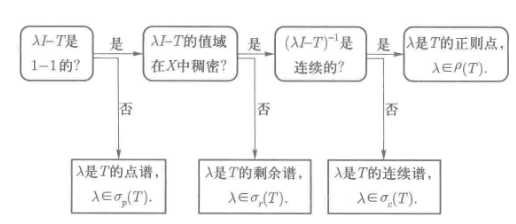
\includegraphics[scale=0.6]{figures/WX20240905-110243@2x.png}
    \caption{$T$的谱集}
\end{figure}

\begin{mdframed}
    \begin{theorem}
        设$H$是\textsl{Hilbert}空间,$T\in \mathcal{B}(H)$,则
        \begin{equation}
            \sigma(T^*)=\{\overline{\lambda}|\lambda\in \sigma(T)\}
        \end{equation}
    \end{theorem}
\end{mdframed}

\textbf{proof.}\hspace*{0.5em} 对$\lambda \in \rho(T)$,
\begin{equation}
    R_{\overline{\lambda}}(T^*)=(\overline{\lambda}I-T^*)^{-1}=[(\lambda I-T)^{-1}]^*=(R_\lambda(T))^T
\end{equation}

\subsection*{\textsl{特征值和特征元素}}

$T$的零空间$\mathcal{N}(\lambda I-T)$称为$T$关于$\lambda$的\textbf{特征子空间},它包括零元素和$T$的全体关于$\lambda$的特征元素,$T$关于$\lambda$的特征子空间的维数$\dim\mathcal{N}(\lambda I-T)$称为
特征值$\lambda$的\textbf{几何重数}。

\begin{example}
    设$H=L^2(-\infty,\infty)$,$T:H\rightarrow H$,$y=Tx$,其中
    \begin{equation}
        y(t)=\int_{\infty}^{t}e^{-(t-\tau)}d\tau
    \end{equation}

  当$\mathcal{D}(T)=H$,$\mathcal{R}(T)\subset H$,当$x(t)=e^{i\omega t}$时
    \begin{eqnarray}
        \int_{-\infty}^{t}e^{-(t-\tau)}e^{i\omega \tau}d\tau=\int_{-\infty}^{t}e^{-t}e^{(1+i\omega)\tau}d\tau=\frac{1}{1+i\omega}e^{i\omega t}
    \end{eqnarray}

    但这并不意味着$1/(1+i \omega)$是算子$T$的连续谱,事实上$x(t)= e^{i\omega t}\notin L^2(-\infty, \infty)$,可以证明$1/(1+i\omega)$是算子$T$的连续谱。
\end{example}

\begin{mdframed}
    \begin{proposition}
        设$\lambda_1,\lambda_2,\cdots,\lambda_n$是线性算子$T$的互不相关的特征值,$x_1,\cdots,x_n$是对应的特征元素,则$x_1,x_2,\cdots, x_n$是线性无关的。
    \end{proposition}
\end{mdframed}

\begin{mdframed}
    \begin{theorem}
        证明:$dim(\mathcal{N}(\lambda I- T))+dim(\mathcal{R}(\lambda I- T))=dim X$
    \end{theorem}
\end{mdframed}

\subsection*{\textsl{闭算子的正则点}}

\begin{mdframed}
    \begin{theorem}
        设$X$是\textsl{Banach}空间,$T$是从$\mathcal{D}(T)\subset X$到$X$的闭线性算子,那么对于所有的$\lambda\in \rho(T)$,
        $(\lambda I-T)^{-1}$是一个定义在全空间上的有界线性算子。
    \end{theorem}
\end{mdframed}

\section{有界线性算子的谱集}

\subsection*{\textsl{有界线性算子的谱集是有界集}}

\begin{mdframed}
    \begin{theorem}
        设$X$是\textsl{Banach空间},$T\in \mathcal{B}(X)$,如果$\Vert T\Vert<1$,则算子$I-T$有有界逆算子,并且
        \begin{equation}
            \begin{aligned}
                & (I-T)^{-1}=\sum^{\infty}_{n=0} T^n \\
                & \Vert (I-T)^{-1}\Vert\leqslant \frac{1}{1-\Vert T\Vert}
            \end{aligned}
        \end{equation}
    \end{theorem}
\end{mdframed}

\begin{mdframed}
    \begin{theorem}
        设$X$是\textsl{Banach空间},$T\in \mathcal{B}(X)$,则$\sigma(T)$是有界集
    \end{theorem}
\end{mdframed}

\subsection*{\textsl{有界线性算子的谱集是闭集}}

\begin{mdframed}
    \begin{theorem}
        设$T$是\textsl{Banach空间}$X$到$X$的线性算子,$\lambda\in \rho(T)$,且$|\mu|<\Vert (\lambda I-T)^{-1}\Vert^{-1}$,则$\lambda+\mu\in \rho(T)$,即$\rho(T)$是一个开集。
    \end{theorem}
\end{mdframed}

\subsection*{\textsl{有界线性算子谱集非空}}

\begin{mdframed}
    \begin{lemma}
        设$\lambda,\mu\in \rho(T)$,
        \begin{equation}
            R_\lambda(T)-R_\mu(T)=(\mu-\lambda)R_{\lambda}(T)R_\mu(T)
        \end{equation}
    \end{lemma}
\end{mdframed}

\begin{mdframed}
    \begin{theorem}
        在正则集$\rho(T)$中,预解式
        \begin{equation}
            R_\lambda(T):\lambda\in \rho(T)\subset \mathbb{C}\rightarrow \mathcal{B}(X)
        \end{equation}

        是关于$\lambda$的算子值解析函数。
    \end{theorem}
\end{mdframed}

\begin{mdframed}
    \begin{theorem}
        设$T$是有界线性算子,则$\sigma(T)\neq \emptyset$
    \end{theorem}
\end{mdframed}

\subsection*{\textsl{有界线性算子的谱半径}}

我们称$r_\sigma(T)=\inf\limits_k\Vert T^k\Vert^{\frac{1}{k}}=\lim\limits_{k\rightarrow \infty}\Vert T^k\Vert^{\frac{1}{k}}$为有界线性算子$T$的\textbf{谱半径}。

\begin{mdframed}
    \begin{theorem}
        设$T\in \mathcal{B}(X)$,则极限
        \begin{equation}
            r_\sigma(T)=\lim_{k\rightarrow\infty}\Vert T^k\Vert^{\frac{1}{k}}=\inf \Vert T^k\Vert^{\frac{1}{k}}
        \end{equation}

        存在
    \end{theorem}
\end{mdframed}

\begin{mdframed}
    \begin{theorem}
        $T\in \mathcal{B}(X)$,则$r_\sigma(T)=\sup\limits_{\lambda\in \sigma(T)}|\lambda|$
    \end{theorem}
\end{mdframed}

\section{有界子共轭线性算子的谱}

\section{紧线性算子的谱}
    \chapter{Exescrise 6}

p393 习题2

p395 习题1,2 
    
%% Prevent urls running into margins in bibliography
\setcounter{biburlnumpenalty}{7000}
\setcounter{biburllcpenalty}{7000}
\setcounter{biburlucpenalty}{7000}

%% Add bibliography
\printbibliography[heading=bibintoc,title=References]

%% ----------------------------------------------------------------------
%%    Appendix (Letters for chapters)
%% ----------------------------------------------------------------------

\appendix

\chapter{Source Code Example}
%\label{chapter:title}

\emph{Adding source code to your report/thesis is supported with the package {\normalfont\texttt{listings}}. An example can be found below. Files can be added using {\normalfont\texttt{\textbackslash lstinputlisting[language=<language>]\{<filename>\}}}.}

\begin{lstlisting}[language=Python]
"""
ISA Calculator: import the function, specify the height and it will return a
list in the following format: [Temperature,Density,Pressure,Speed of Sound].
Note that there is no check to see if the maximum altitude is reached.
"""

import math
g0 = 9.80665
R = 287.0
layer1 = [0, 288.15, 101325.0]
alt = [0,11000,20000,32000,47000,51000,71000,86000]
a = [-.0065,0,.0010,.0028,0,-.0028,-.0020]

def atmosphere(h):
    for i in range(0,len(alt)-1):
        if h >= alt[i]:
            layer0 = layer1[:]
            layer1[0] = min(h,alt[i+1])
            if a[i] != 0:
                layer1[1] = layer0[1] + a[i]*(layer1[0]-layer0[0])
                layer1[2] = layer0[2] * (layer1[1]/layer0[1])**(-g0/(a[i]*R))
            else:
                layer1[2] = layer0[2]*math.exp((-g0/(R*layer1[1]))*(layer1[0]-layer0[0]))
    return [layer1[1],layer1[2]/(R*layer1[1]),layer1[2],math.sqrt(1.4*R*layer1[1])]
\end{lstlisting}

\chapter{Task Division Example}
%\label{chapter:title}

\emph{If a task division is required, a simple template can be found below for convenience. Feel free to use, adapt or completely remove.}

\begin{table}[htb]
    \setlength\extrarowheight{4pt}
    \centering
    \caption{Distribution of the workload}
    \label{tab:taskdivision}
    \begin{tabularx}{\textwidth}{lXX}
        \toprule
        & Task & Student Name(s) \\
        \midrule
        & Summary & \\
        Chapter 1 & Introduction &  \\
        Chapter 2 &  & \\
        Chapter 3 &  & \\
        Chapter * &  & \\
        Chapter * & Conclusion &  \\
        \midrule
        & Editors & \\
        & CAD and Figures & \\
        & Document Design and Layout & \\
        \bottomrule
    \end{tabularx}
\end{table}

%\chapter{Cauchy-Schwarz不等式\\及其证明}

\section{定理描述}

\subsection*{一般形式}

Cauchy-Schwarz不等式的一般描述如下
\begin{theorem}
    已知$a_1,\cdots,a_n,b_1\cdots,b_n$是实数,则
    \begin{equation}
        (\sum\limits_{i=1}^{n}a_ib_i)^2\leqslant (\sum\limits_{i=1}^{n}a^2_i)(\sum\limits_{i=1}^{n}b^2_i) 
    \end{equation}

    等号成立的充分必要条件是
    \begin{equation}
        a_i=\lambda b_i,\ \ i=1,\cdots n
    \end{equation}
\end{theorem}

\subsection*{推广到复数形式}
不等式可以推广到复数。如何推广呢?不等式只有在实数时才有意义,对于复数则需要考虑角度和模长
大小关系。

\begin{theorem}
    已知$a_1,\cdots,a_n,b_1\cdots,b_n$是复数,则
    \begin{equation}
        |\sum\limits_{i=1}^{n}a_ib_i|^2\leqslant (\sum\limits_{i=1}^{n}|a_i|^2)(\sum\limits_{i=1}^{n}|b_i|^2) 
    \end{equation}

    等号成立的充分必要条件是
    \begin{equation}
        a_i=\lambda b_i,\ \ i=1,\cdots n
    \end{equation}
\end{theorem}

\subsection*{矩阵形式}

根据线性代数的理论:\textsl{任意正定对称矩阵都可以定义内积}。因此若$A=a_{ij}$为正定对称矩阵,则
$Cauchy$不等式存在
\begin{theorem}
    已知$(a_{ij})_{kl}$是正定对称矩阵,对于$x_1,\cdots,x_n,y_1.\cdots,y_n$是任意复数或者实数,则
    \begin{equation}
        |\sum\limits_{i=1}^{n}a_{ij}x_iy_j|\leqslant \sqrt{\sum\limits_{i,j=1}^{n}a_{ij}x_ix_j}
        \sqrt{\sum\limits_{i,j=1}^{n}a_{ij}y_iy_j}
    \end{equation}

    等号成立的充分必要条件是
    \begin{equation}
        a_i=\lambda b_i,\ \ i=1,\cdots n
    \end{equation}
\end{theorem}

\subsection*{无穷级数形式}

\begin{theorem}
    已知$a_1,\cdots,a_n,\cdots,b_1\cdots,b_n,\cdots$是复数,则
    \begin{equation}
        |\sum\limits_{i=1}^{\infty}a_ib_i|\leqslant 
        (\sum\limits_{i=1}^{\infty}|a_i|^2)^{\frac{1}{2}}
        (\sum\limits_{i=1}^{\infty}|b_i|^2)^{\frac{1}{2}}
    \end{equation}

    等号成立的充分必要条件是
    \begin{equation}
        a_i=\lambda b_i,\ \ i=1,\cdots ;\ \ \lambda\in \mathbb{C}
    \end{equation}
    \begin{equation}
        \sum\limits_{i=1}^{\infty}|a_i|^2<\infty
    \end{equation}
    \begin{equation}
        \sum\limits_{i=1}^{\infty}|b_i|^2<\infty
    \end{equation}
\end{theorem}

\subsection*{积分形式}

\begin{theorem}
    已知$f,g$是区间$[a,b]$上的连续函数,$f,g\in C[a,b]$,则
    \begin{equation}
        |\int_{a}^{b}f(x)g(x)dx|^2\leqslant \int_{a}^{b}|f(x)|^2dx \int_{a}^{b}|g(x)|^2dx 
    \end{equation}
\end{theorem}

\subsection*{$H\ddot{o}lder$不等式}
\begin{theorem}
    已知$a_1,\cdots,a_n,b_1\cdots,b_n$是复数,$p,q\geqslant 1$,$\frac{1}{p}+\frac{1}{q}=1$,则
    \begin{equation}
        |\sum\limits_{i=1}^{n}a_ib_i|\leqslant (\sum\limits_{i=1}^{n}|a_i|^p)^{\frac{1}{p}}
        (\sum\limits_{i=1}^{n}|b_i|^q)^{\frac{1}{q}} 
    \end{equation}
\end{theorem}

\subsection*{广义Cauchy-Schwarz不等式}

\begin{theorem}
    一般$n$维向量空间中的Cauchy-Schwarz不等式形式为
    \begin{equation}
        |a\cdot b|\leqslant \Vert a\Vert \Vert b\Vert
    \end{equation}
\end{theorem}

\section{余弦定律}
考虑三角形$\bigtriangleup ABC$,三条边的分量分别是
\begin{equation}
    \overrightarrow{a}=\overrightarrow{AB},\overrightarrow{b}=\overrightarrow{AC},
    \overrightarrow{c}=\overrightarrow{CB}=\vec{a}-\vec{b}
\end{equation}

\begin{figure}[H]
    \centering
    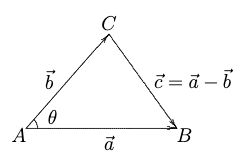
\includegraphics[scale=0.6]{figures/余弦定律.png}
    \caption{余弦定律}
\end{figure}

根据余弦定律$|\vec{a}|^2+|\vec{b}|^2-|\vec{a}-\vec{b}|^2=2|\vec{a}||\vec{b}|\cos{\theta}$以及余弦的性质$|\cos{\theta}|\leqslant 1$,可得
\begin{equation}
    |\vec{a}\cdot\vec{b}|\leqslant |\vec{a}||\vec{b}|
\end{equation}

这就是Cauchy-Schwarz不等式。他告诉我们Cauchy-Schwarz不等式的几何意义:三角形两边的内积小于两个向量长度的乘积。

\section{证明}

考虑$b$在$a$上的投影之差的最短距离,设
\begin{equation}
    \overrightarrow{c}=\vec{b}-\lambda \vec{a},\ \ \ \ \lambda\in \mathbb{R}
\end{equation}

$\vec{c}$的长度

\begin{eqnarray}
    |\vec{c}|^2=\vec{c}\cdot \vec{c}=|\vec{a}|^2\lambda^2+2\vec{a}\cdot \vec{b}\lambda +|b|^2>0
\end{eqnarray}

上式可视为$\lambda$的二次方程,且与$\lambda$轴没有交点

\begin{equation}
    \bigtriangleup = (2\vec{a}\vec{b})^2-4|\vec{a}|^2|\vec{b}|^2\leqslant 0
\end{equation}

因此有
\begin{equation}
    |\vec{a}\cdot \vec{b}|\leqslant |\vec{a}||\vec{b}|
\end{equation} % Create file to add

\end{document}
